% Created by tikzDevice version 0.10.1 on 2017-07-05 01:07:09
% !TEX encoding = UTF-8 Unicode
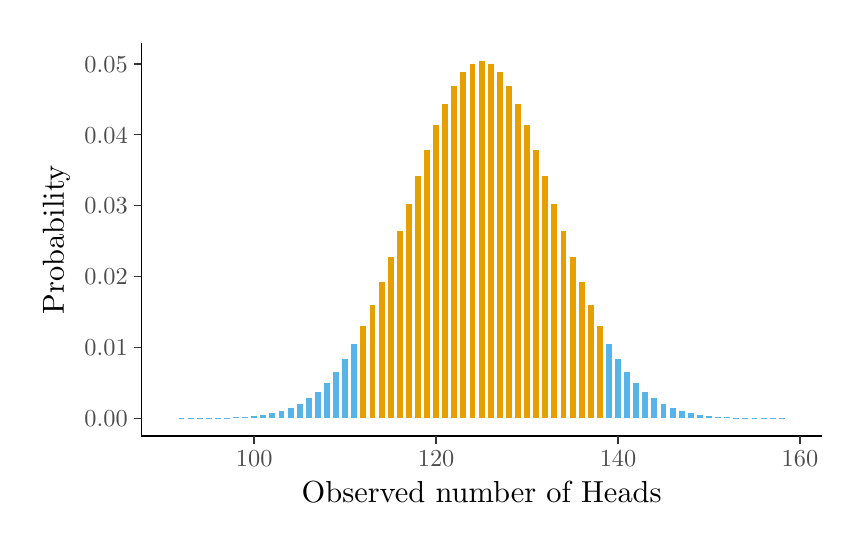
\begin{tikzpicture}[x=1pt,y=1pt]
\definecolor{fillColor}{RGB}{255,255,255}
\path[use as bounding box,fill=fillColor,fill opacity=0.00] (0,0) rectangle (292.45,178.21);
\begin{scope}
\path[clip] (  0.00,  0.00) rectangle (292.45,178.21);
\definecolor{drawColor}{RGB}{255,255,255}
\definecolor{fillColor}{RGB}{255,255,255}

\path[draw=drawColor,line width= 0.6pt,line join=round,line cap=round,fill=fillColor] (  0.00,  0.00) rectangle (292.45,178.21);
\end{scope}
\begin{scope}
\path[clip] ( 41.11, 30.56) rectangle (286.95,172.71);
\definecolor{fillColor}{RGB}{255,255,255}

\path[fill=fillColor] ( 41.11, 30.56) rectangle (286.95,172.71);
\definecolor{fillColor}{RGB}{86,180,233}

\path[fill=fillColor] ( 54.50, 37.02) rectangle ( 56.64, 37.04);

\path[fill=fillColor] ( 57.79, 37.02) rectangle ( 59.93, 37.05);

\path[fill=fillColor] ( 61.08, 37.02) rectangle ( 63.21, 37.08);

\path[fill=fillColor] ( 64.36, 37.02) rectangle ( 66.50, 37.11);

\path[fill=fillColor] ( 67.65, 37.02) rectangle ( 69.79, 37.17);

\path[fill=fillColor] ( 70.94, 37.02) rectangle ( 73.07, 37.26);

\path[fill=fillColor] ( 74.22, 37.02) rectangle ( 76.36, 37.39);

\path[fill=fillColor] ( 77.51, 37.02) rectangle ( 79.65, 37.59);

\path[fill=fillColor] ( 80.80, 37.02) rectangle ( 82.93, 37.88);

\path[fill=fillColor] ( 84.08, 37.02) rectangle ( 86.22, 38.30);

\path[fill=fillColor] ( 87.37, 37.02) rectangle ( 89.51, 38.88);

\path[fill=fillColor] ( 90.66, 37.02) rectangle ( 92.79, 39.70);

\path[fill=fillColor] ( 93.94, 37.02) rectangle ( 96.08, 40.81);

\path[fill=fillColor] ( 97.23, 37.02) rectangle ( 99.37, 42.28);

\path[fill=fillColor] (100.52, 37.02) rectangle (102.65, 44.22);

\path[fill=fillColor] (103.80, 37.02) rectangle (105.94, 46.71);

\path[fill=fillColor] (107.09, 37.02) rectangle (109.23, 49.85);

\path[fill=fillColor] (110.38, 37.02) rectangle (112.51, 53.73);

\path[fill=fillColor] (113.66, 37.02) rectangle (115.80, 58.44);

\path[fill=fillColor] (116.95, 37.02) rectangle (119.09, 64.04);
\definecolor{fillColor}{RGB}{230,159,0}

\path[fill=fillColor] (120.24, 37.02) rectangle (122.37, 70.55);

\path[fill=fillColor] (123.52, 37.02) rectangle (125.66, 77.97);

\path[fill=fillColor] (126.81, 37.02) rectangle (128.95, 86.24);

\path[fill=fillColor] (130.10, 37.02) rectangle (132.23, 95.22);

\path[fill=fillColor] (133.38, 37.02) rectangle (135.52,104.76);

\path[fill=fillColor] (136.67, 37.02) rectangle (138.81,114.60);

\path[fill=fillColor] (139.96, 37.02) rectangle (142.09,124.46);

\path[fill=fillColor] (143.24, 37.02) rectangle (145.38,134.01);

\path[fill=fillColor] (146.53, 37.02) rectangle (148.66,142.90);

\path[fill=fillColor] (149.82, 37.02) rectangle (151.95,150.78);

\path[fill=fillColor] (153.10, 37.02) rectangle (155.24,157.31);

\path[fill=fillColor] (156.39, 37.02) rectangle (158.52,162.20);

\path[fill=fillColor] (159.67, 37.02) rectangle (161.81,165.22);

\path[fill=fillColor] (162.96, 37.02) rectangle (165.10,166.25);

\path[fill=fillColor] (166.25, 37.02) rectangle (168.38,165.22);

\path[fill=fillColor] (169.53, 37.02) rectangle (171.67,162.20);

\path[fill=fillColor] (172.82, 37.02) rectangle (174.96,157.31);

\path[fill=fillColor] (176.11, 37.02) rectangle (178.24,150.78);

\path[fill=fillColor] (179.39, 37.02) rectangle (181.53,142.90);

\path[fill=fillColor] (182.68, 37.02) rectangle (184.82,134.01);

\path[fill=fillColor] (185.97, 37.02) rectangle (188.10,124.46);

\path[fill=fillColor] (189.25, 37.02) rectangle (191.39,114.60);

\path[fill=fillColor] (192.54, 37.02) rectangle (194.68,104.76);

\path[fill=fillColor] (195.83, 37.02) rectangle (197.96, 95.22);

\path[fill=fillColor] (199.11, 37.02) rectangle (201.25, 86.24);

\path[fill=fillColor] (202.40, 37.02) rectangle (204.54, 77.97);

\path[fill=fillColor] (205.69, 37.02) rectangle (207.82, 70.55);
\definecolor{fillColor}{RGB}{86,180,233}

\path[fill=fillColor] (208.97, 37.02) rectangle (211.11, 64.04);

\path[fill=fillColor] (212.26, 37.02) rectangle (214.40, 58.44);

\path[fill=fillColor] (215.55, 37.02) rectangle (217.68, 53.73);

\path[fill=fillColor] (218.83, 37.02) rectangle (220.97, 49.85);

\path[fill=fillColor] (222.12, 37.02) rectangle (224.26, 46.71);

\path[fill=fillColor] (225.41, 37.02) rectangle (227.54, 44.22);

\path[fill=fillColor] (228.69, 37.02) rectangle (230.83, 42.28);

\path[fill=fillColor] (231.98, 37.02) rectangle (234.12, 40.81);

\path[fill=fillColor] (235.27, 37.02) rectangle (237.40, 39.70);

\path[fill=fillColor] (238.55, 37.02) rectangle (240.69, 38.88);

\path[fill=fillColor] (241.84, 37.02) rectangle (243.98, 38.30);

\path[fill=fillColor] (245.13, 37.02) rectangle (247.26, 37.88);

\path[fill=fillColor] (248.41, 37.02) rectangle (250.55, 37.59);

\path[fill=fillColor] (251.70, 37.02) rectangle (253.84, 37.39);

\path[fill=fillColor] (254.99, 37.02) rectangle (257.12, 37.26);

\path[fill=fillColor] (258.27, 37.02) rectangle (260.41, 37.17);

\path[fill=fillColor] (261.56, 37.02) rectangle (263.70, 37.11);

\path[fill=fillColor] (264.85, 37.02) rectangle (266.98, 37.08);

\path[fill=fillColor] (268.13, 37.02) rectangle (270.27, 37.05);

\path[fill=fillColor] (271.42, 37.02) rectangle (273.56, 37.04);
\end{scope}
\begin{scope}
\path[clip] (  0.00,  0.00) rectangle (292.45,178.21);
\definecolor{drawColor}{RGB}{0,0,0}

\path[draw=drawColor,line width= 0.6pt,line join=round] ( 41.11, 30.56) --
	( 41.11,172.71);
\end{scope}
\begin{scope}
\path[clip] (  0.00,  0.00) rectangle (292.45,178.21);
\definecolor{drawColor}{gray}{0.30}

\node[text=drawColor,anchor=base east,inner sep=0pt, outer sep=0pt, scale=  0.88] at ( 36.16, 33.99) {0.00};

\node[text=drawColor,anchor=base east,inner sep=0pt, outer sep=0pt, scale=  0.88] at ( 36.16, 59.62) {0.01};

\node[text=drawColor,anchor=base east,inner sep=0pt, outer sep=0pt, scale=  0.88] at ( 36.16, 85.26) {0.02};

\node[text=drawColor,anchor=base east,inner sep=0pt, outer sep=0pt, scale=  0.88] at ( 36.16,110.89) {0.03};

\node[text=drawColor,anchor=base east,inner sep=0pt, outer sep=0pt, scale=  0.88] at ( 36.16,136.53) {0.04};

\node[text=drawColor,anchor=base east,inner sep=0pt, outer sep=0pt, scale=  0.88] at ( 36.16,162.16) {0.05};
\end{scope}
\begin{scope}
\path[clip] (  0.00,  0.00) rectangle (292.45,178.21);
\definecolor{drawColor}{gray}{0.20}

\path[draw=drawColor,line width= 0.6pt,line join=round] ( 38.36, 37.02) --
	( 41.11, 37.02);

\path[draw=drawColor,line width= 0.6pt,line join=round] ( 38.36, 62.65) --
	( 41.11, 62.65);

\path[draw=drawColor,line width= 0.6pt,line join=round] ( 38.36, 88.29) --
	( 41.11, 88.29);

\path[draw=drawColor,line width= 0.6pt,line join=round] ( 38.36,113.92) --
	( 41.11,113.92);

\path[draw=drawColor,line width= 0.6pt,line join=round] ( 38.36,139.56) --
	( 41.11,139.56);

\path[draw=drawColor,line width= 0.6pt,line join=round] ( 38.36,165.19) --
	( 41.11,165.19);
\end{scope}
\begin{scope}
\path[clip] (  0.00,  0.00) rectangle (292.45,178.21);
\definecolor{drawColor}{RGB}{0,0,0}

\path[draw=drawColor,line width= 0.6pt,line join=round] ( 41.11, 30.56) --
	(286.95, 30.56);
\end{scope}
\begin{scope}
\path[clip] (  0.00,  0.00) rectangle (292.45,178.21);
\definecolor{drawColor}{gray}{0.20}

\path[draw=drawColor,line width= 0.6pt,line join=round] ( 81.86, 27.81) --
	( 81.86, 30.56);

\path[draw=drawColor,line width= 0.6pt,line join=round] (147.60, 27.81) --
	(147.60, 30.56);

\path[draw=drawColor,line width= 0.6pt,line join=round] (213.33, 27.81) --
	(213.33, 30.56);

\path[draw=drawColor,line width= 0.6pt,line join=round] (279.06, 27.81) --
	(279.06, 30.56);
\end{scope}
\begin{scope}
\path[clip] (  0.00,  0.00) rectangle (292.45,178.21);
\definecolor{drawColor}{gray}{0.30}

\node[text=drawColor,anchor=base,inner sep=0pt, outer sep=0pt, scale=  0.88] at ( 81.86, 19.55) {100};

\node[text=drawColor,anchor=base,inner sep=0pt, outer sep=0pt, scale=  0.88] at (147.60, 19.55) {120};

\node[text=drawColor,anchor=base,inner sep=0pt, outer sep=0pt, scale=  0.88] at (213.33, 19.55) {140};

\node[text=drawColor,anchor=base,inner sep=0pt, outer sep=0pt, scale=  0.88] at (279.06, 19.55) {160};
\end{scope}
\begin{scope}
\path[clip] (  0.00,  0.00) rectangle (292.45,178.21);
\definecolor{drawColor}{RGB}{0,0,0}

\node[text=drawColor,anchor=base,inner sep=0pt, outer sep=0pt, scale=  1.10] at (164.03,  6.47) {Observed number of Heads};
\end{scope}
\begin{scope}
\path[clip] (  0.00,  0.00) rectangle (292.45,178.21);
\definecolor{drawColor}{RGB}{0,0,0}

\node[text=drawColor,rotate= 90.00,anchor=base,inner sep=0pt, outer sep=0pt, scale=  1.10] at ( 13.08,101.63) {Probability};
\end{scope}
\end{tikzpicture}
